\documentclass[a4paper,11pt]{article}
\usepackage[utf8]{inputenc}

%% Useful packages
\usepackage{amsmath}
\usepackage{amsthm}
\usepackage{amssymb}
\usepackage{graphicx}
\usepackage[colorinlistoftodos]{todonotes}
\usepackage[colorlinks=true, allcolors=blue]{hyperref}
\usepackage[a4paper]{geometry} % Pour modifier les marges
\geometry{hscale=0.7,vscale=0.7,centering}

\title{Sensim: Sensor Extremelly Naturally Simulated In our Model (or just Sensor Simulation)}
\author{Simon Fernandez, Mathieu Vavrille}
\date{December 2018}


\def\noteSimon#1{\marginpar{\textcolor{blue}{#1}}}
\def\noteMathieu#1{\marginpar{\textcolor{red}{#1}}}

\begin{document}

\maketitle

\begin{abstract}
  This project is a helper to create simulation of sensors. The goal is to model a place composed of many sensors (smart city, smart campus), and simulate the behavior of all the sensors. The implementation is done using Python (3), and the created language is an embedded language.
\end{abstract}


\section{General model}




The general model is divided into three main components:
\begin{itemize}
\item Simulation
\item Display
\item Sensor
\end{itemize}

There are also secondary components used to encapsulate data and time through
the simulation : \emph{Data} and \emph{Timestamp}. These two classes will be
used by the other components.

Figure \ref{meta-meta-model} shows the links between the different components
of the general model.

\begin{figure}
  \centering
  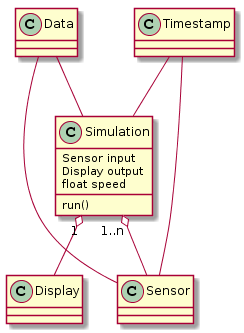
\includegraphics[scale = 0.5]{figures/meta-meta-model.png}
  \label{meta-meta-model}
  \caption{The general model}
\end{figure}

\subsection{Simulation}

The simulation is the core class that will run the simulation. In this class,
the user should be able to define the speed at with he wants to run the
simulation (for example run a simulation twice as fast as it should be). He
will also define the sensors that will be used, and the display where whe wants
to output the data.

Once the different components of the model are given, the user may start the
simulation. The \emph{Simulation} class will then handle time, ask the sensors
for data, and send it to the given display.

\subsection{Display}

This class will deal with the output of the simulation. Many different outputs
can be defined: CSV, JSON formats, or outputing in an influxDB database (that
can be then visualised with Grafana).

The Display is plugged to the simulation and will receive the generated data
as soon as they are generated during the simulation.


\subsection{Sensor}

This is the most base class that will allow the user to define sensors. The
model provides different kinds of predefined Sensors in order to help the user
to easily build their simulation.

Even if different kinds of sensors exist, they must all behave the same
way. Because of this, the Simulation does not have to know what kind of sensors
it is handling.

\subsection{Generator}

Some sensors may be complex to build. If they are an aggregation of many
sensors, or implement complex functions. In order to provide an easy way to
build complex sensors, we made this Generator class. It can be seen as a Sensor
in construction. The user will progressively give data to the Constructor, give
it all the information it needs, and when all options are given, the Generator
will output a Sensor behaving like the user wants.

This is why it is important for all Sensors to behave the same way : the user
does not care how the Sensor behaves internaly, the important information is
the data output. Generators are here to help build Sensors. But they are not
mandatory, the user can build the sensors by hand.

\subsection{Timestamp}

The Timestamp class is here to provide a more friendly interface for
time. There are different kinds of times : absolute dates, relative dates,
durations, ... In order to provide a clean access to all these possibilities,
the Timestamp class tries to overload all basic operations so that time can
be smoothly used in user-defined functions. For example, when one wants a
"function that is a second order polynomial in time", is time an absolute
time (total seconds since Epoch) ? Is it time elapsed since the begining of
the simulation ? Is it a function of the "hour" field of a date ?

The Timestamp allows to access all these informations and use them smoothly.

\subsection{Data}

The Data class will represent a point of data generated by a sensor. It
encapsulates all informations that are needed to describe a piece of
information. It contains the Timestamp when this data was generated, the name
of the sensor that generated it, the value of the data, and all other field
that may be used to describe the data.

This class will not be used by the user but it will be necessary for the
simulation.



\section{How to use the language}



The class diagram of the implementation is done in the appendix.

\subsection{Creating the model}

First, the user needs to create the set of sensors that are in their model.
Each sensor has type $\texttt{Sensor()}$. This class is an abstract class.
The user must use sub-classes that define different behaviours.

Each Sensor have a given name. If the name is not defined when building the
sensor, a pre-generated unique name will be used.

There are three kinds of $\texttt{Sensor(name)}$.

\subsubsection{$\texttt{Importer(name)}$}
They are used to get data already generated and stored in different formats
\begin{itemize}
    \item $\texttt{JSONImporter(name, filename)}$ : Reads the JSON file named
        $filename$ and outputs the data contained in it. It must contain the
        following fields:
        \begin{itemize}
            \item "bn" : Name of the sensor
            \item "e" : list of data : each piece of data contains two fields:
            \item "t" : Timestamp when the data was generated
            \item "v" : Value of the sensor at time "t"
        \end{itemize}
    \item $\texttt{csvImporter(name, filename)}$ : Reads the CSV file named
        $filename$ and outputs the data contained in it. The first column must
        be the timestamp. The rest of the columns will be added in the custom
        fields of the \emph{Data} object.
\end{itemize}

\subsubsection{$\texttt{ModelSensor(name, step)}$}
Generates data following a given behaviour. Data is generated on-the-fly. A
value is generated after each $step$ amount of time.

There are some pre-defined $\texttt{ModelSensor()}$.

\begin{itemize}
    \item $\texttt{FunctionSensor(name, step, function)}$ : $function$ is a
python function that will be called on each time step. This allows to use Python
functions, and external modules (for example, call the $np.sin$ function from
the numpy module).
    \item $\texttt{PolynomialSensor(name, step, polynomial, coefs, points)}$ : a
special case of $\texttt{FunctionSensor}$. It implements a polynomial function.
There are three ways to define a polynomial sensor :
    \begin{itemize}
        \item $polynomial$: give the polynomial function
        \item $coefs$: give the array of the coefficients of the polynomial
        \item $points$: give a list of $(x, y)$ values, interpolates the
        polynomial fitting these points
    \end{itemize}
    \item $\texttt{MarkovChain()}$: A Markov chain : use the $\texttt{addState}$,
    $\texttt{addTransition}$ and $\texttt{setStartNode}$ to define a custom chain.
    At each time step, it will compute a transition following the given
    probabilities, and send the new state.
\end{itemize}

\subsubsection{Wrappers}
Modify the behaviour of $sensor$ it contains. It is a wrapper that can catch the
returned data and apply operations on it.

There are three kinds of Wrappers for now:
\begin{itemize}
    \item $\texttt{MaskerSensor(name, sensor, start, stop)}$: forwards the data
of $sensor$ only if the timestamp is between $start$ and $stop$. This allows to
"hide" the sensor during some time, or activate it only on a given period.
    \item $\texttt{SpeedSensor(name, sensor, factor)}$: scales the speed of
$sensor$ by factor $factor$. This allows to set a sensor to run twice as fast,
or twice as slow.
    \item $\texttt{AggregatedSensor(name, sensors)}$: encapsulates a set of
$sensors$. It gathers the data from all $sensors$ and sends them, like a funnel.
\end{itemize}

\subsection{User-friendly ways to define sensors}

Some functions are added to help the user build Sensors. Each function returns
the builded sensor, so they can be stacked.
If $s$ and $s'$ are sensors,
\begin{itemize}
    \item $\texttt{s.named(name)}$ : changes the name of the sensor
    \item $\texttt{s.turnedOnAt(time)}$: disables the sensor before $time$
    \item $\texttt{s.turnedOffAt(time)}$: disables the sensor after $time$.
$time$ can be an absolute time, or a relative time (relative to the start time
of the sensor)
    \item $\texttt{s.turnedOnBetween(start, stop))}$: both at the same time
    \item $s + s'$: builds a sensor sending the data of both sensors
    \item $s * n$ with $n$ an integer : builds a sensor containing $n$ copies
of $s$
\end{itemize}

So, if $s$ models the sensor of a parking slot, $(s*30).named("parking")$ is a
sensor containing 30 independent parking slots, and returning the data of each
slot. This multiple sensor is called "parking"

\subsection{Preparing the display devices}
Displays the simulated data to a format where it will be visualised.

\begin{itemize}
    \item $\texttt{InfluxDBDisplay(url)}$ : outputs the data to an influxDB data
base running at url $url$
    \item $\texttt{JSONDisplay(filename)}$ : outputs the data in a JSON file
called $filename$
\end{itemize}


\subsection{Creating the simulation}
The $\texttt{Simulation}$ object is built with all the previous objects:
$\texttt{Simulation(name, display, sensors, speed, start, stop, realtime)}$

\begin{itemize}
    \item $name$ : name of the simulation
    \item $display$ : the display where to export the data
    \item $sensors$ : list of the sensors to simulate
    \item $speed$ : speed factor to speed up or slow down the whole simulation
    \item $start$ : timestamp when the simulation starts
    \item $stop$ : timestamp when the simulation ends
    \item $realtime$ : if $True$, the simulation will wait and make sure the
data is generated at the good timestamp, nothing will be pre computed.
\end{itemize}

Once the simulation $simu$ is defined, a simple $simu.run()$ will start the
simulation.

\subsection{Examples}
The easiest way to discover how to build the simulation is to look at the
examples given in the folder, they depict most of the functionnalities.





\section{Concrete implementation}



In this section, we will present how we implemented everything. The presentation will be done class by class. All the functions that are prefixed by an underscore should never be used by the user (for example \_popNext). These functions are auxilliary functions that are used by the simulation to generate the data. This convention follows the PEP8 convention of python, as python does not give a way to protect methods.

\subsection{Sensors}

The main class that need to be understood first is the class of the sensors. The idea is to have sensors defined by different manners that will behave the same way. For example, from the simulation class, it will be impossible to know if a data comes from data imported from a file, or from a Markov Chain. The Sensor class is an abstract class that will define the functions that need to be implemented in order to get this behaviour.

\subsubsection{The Sensor abstract class}

The main implementation choice that was made was the one to know how we would generate the data, and send it to the simulation. This is done using a method \verb!_popNext! that will return the next data generated by the sensor. The associated function is \verb!_getNext! that will return the next data that will be generated, but this data is not meant to be used right now (the data can be used to know beforehand when will be the next data generated).

Above that, a sensor have a \verb!name! and a \verb!speed! attributes, with the associated setters (\verb!setName! and \verb!setSpeed!). If the name is not defined by the user, it will be generated automatically as ``Sensor\_i'' where $i$ will be incremented each time a new name is defined (to prevent from two sensors with the same name).
\noteMathieu{Is the speed still useful ?}

Now we should look deeper into the different classes that will inherit from the Sensor class

\subsubsection{The Importer abstract class}

The importer class is also an abstract class that implements the function to read text from an input file. The user have to define a filename at the creation of the class. The real importation of the data (depending on the type of storage of the data) is done in inherited classes.

\paragraph{The JsonImporter class}




\subsubsection{The modelSensor abstract class}

This class is an abstract class that represent a sensor modelled by some law. For example, the user may want to define a sensor that will behave like a Markov Chain, or a like a given function. The inherited class will represent a different model. There is an attribute defined by the modelSensor class that is the step of the created sensor. The step attribute will define at which speed the sensor will send data (for example, a computer energy consumption can be received each millisecond, whereas sensor from a parking lot will only send data every second, or minute).

\paragraph{Markov Chains}

One model that is implemented is the one of Markov Chains. The state returned by the sensor is following the low of a Markov Chain. To define a Markov Chain, the user need to define the nodes, the transitions and the starting node. Adding nodes and setting the starting node is easy, the nodes are the values that will be returned by the sensor: for example, if the nodes are integers (modelling the wealth of someone) it will be possible to show it on a graph; the nodes can also be strings (modelling the weather: ``sunny'', ``rainy'', ``snowy'') and then, it will be harder to show the data on a graph.

Setting the transition is harder: the implementation choosed to give a method \verb!addTransition(node1, node2, proba)!. The user have to define all the values of the transitions (the initial probability is 0).

The Markov Chains come with a big issue that are the fact that we use probabilities. The next state of the MC is a random variable, that need to follow a distribution (where the sum of the probabilities is equal to 1). If the user don't specify well the probability of the transitions, this can lead to bugs. The solution that was done was to enforce that the last node have probability equal to one minus the sum of the other probabilities. This way, even if the user enters an illegal probability distribution, the simulation will work.
This was also done because as we are working with probabilities, we work with floating points. The issue with floating points is that some errors of roundings can occur, even if the user entered a legitimate distribution (for example [0.01, 0.01, ..., 0.01] that are not dyadic numbers). This is very unlikely to happen, but it is possible

\paragraph{FunctionSensor class}

This class will also behave like a sensor, but will generate data from a given function. The function is an attribute of the instance of the class, and there is the setter associated to it.

\subparagraph{Polynomial sensor}

\paragraph{Masked Sensor}

\noteMathieu{TODO Simon!}


\subsection{Display}

The display is the third big block of the whole simulation. It will output data on different possible outputs. Currently, two types of output are implemented: display to an influxDB database, and to a file in JSON format.

\subsubsection{The Display abstract class}

This class is really here to define the interface that will be used by the simulation. This interface contains the methods \verb!addPlot!, \verb!_setup! and \verb!end!. The method addPlot will add a data in the output. The method end will be called by the simulation when there is no more data to send; this is used by displays in files, because we don't want to open and close the file each time we add a data in the file. To do this, we just open the file at the end of the simulation, write everything, and close right after.

\subsubsection{Display to an influxDB database}

\subsubsection{Display to a file in JSON format}




\section{Possible improvements}

This section presents the improvements that can be done to the project. The
improvements presented are not implemented because of a lack of time, or
knowledge of the domain. The improvements are presented component by component.

\subsection{Markov Chain}

\label{improvement_MC}

The way to define Markov Chains is currently a little unintuitive for the
user. The user adds the nodes, and the starting node (which is fine), but the
issue comes when defining the transition matrix. The current implementation
uses the function \verb!addTransition()!.

This can be improved because it is tedious to define each transition by
hand. One could improve it by giving a function \verb!addOneTransition(node,transition)! where the transition parameter is a dictionary containing
the probability for each associated key. To be even faster, one could add a
function to define the whole transition matrix in one time, with a dictionnary
contaning the transition for each associated node.

The python dictionaries seems to be a good way to do it because they really
show the fact that the keys and the values are associated. Then it will be
translated to a real transition matrix, which is less user-friendly, but more
programmer-friendly.


\subsection{JsonImporter}

\label{imprevoment_jsonimporter}

The current implementation of the JsonImporter class does not give
possibilities for other key names in the dictionary. The key \verb!"bn"! have
to contain the name of the sensor, as well as the other forced keys. This
suppositions were done because we saw on examples that it was one way to
represent data from sensors.

To improve this importer, one can allow the user to specify how is the file
loaded. Json files have a tree structure where nodes are given by types,
links of the tree are given by keys (of dictionaries) or indices (of lists),
and leaves of the tree are data of the file. By specifying the structure of the
tree, the user would be able to have personalized json files.

With that, we should have predefined tree structures (for example, the one
that is already implemented). This way, one could implement all the main json
structures for sensor outputs, and make them available to the user.



\appendix

\section{Class diagrams}



\begin{figure}
  \centering
  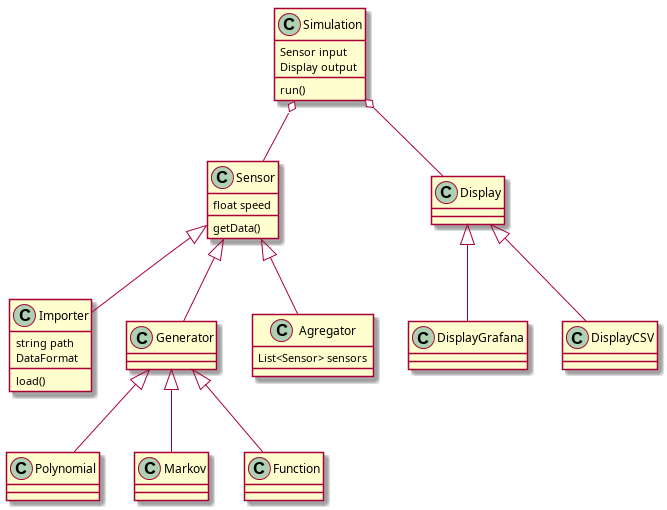
\includegraphics[scale = 0.45]{figures/meta-model.png}
  \label{meta-model_fig}
  \caption{Class diagram showing the hierarchy of the project}
\end{figure}

\end{document}
